En este capítulo se justifica y se describe la metodología de desarrollo sobre la que se apoya el proceso de ingeniería. En este proyecto se ha empleado una metodología ágil, Scrum. Se ha optado por esta solución frente a otras clásicas como la de proceso unificado porque al usar un modelo incremental, basado en iteraciones, aseguramos que al final de cada etapa tengamos un producto operativo y que en sucesivas etapas se irá completando.



\section{Scrum}

El Scrum es un proceso de la Metodología Ágil que se usa para minimizar los riesgos durante la realización de un proyecto. 
Esta metodología esta basada en ciclo iterativos lo que se traduce en una gran flexibilidad a la hora de adaptarse a cambios en el proyecto o sobre el control de riesgos. 



Entre las ventajas se encuentran la productividad, calidad y que se realiza un seguimiento diario de los avances del proyecto, logrando que los integrantes estén unidos, comunicados. Esta cualidad no será palpable ya que en el caso de este proyecto el equipo estará formado por una sola persona.\\

\subsection{Sprint}

Por Sprint entendemos un bloque de tiempo fijo de entorno a 1 mes en el que
se crea una version de nuestra aplicación que se irá incrementando de tamaño
según van avanzando los Sprints. Los Sprints se pueden considerar como pequeños
proyectos ya que al final de cada uno de ellos debemos tener un producto
operativo, es decir, que responda a la historia o historias planteadas en él.



\subsection{Participantes}
\begin{itemize}
\item \textbf{Product Owner}\\
Habla por el cliente, y asegura que el equipo cumpla las expectativas. Es “el jefe”, sus decisiones deben ser
respectadas y acatadas. Estas  decisiones influirán en la prioridad de la lista de tareas o Product Backlog.



\item \textbf{Scrum Master}\\
Es el encargado de liderar la reuniones y ayudar al equipo en los problemas que tengan. Debe minimizar las imposibilidades que surgen en el desarrollo del proyecto para que se cumplan los objetivos del Sprint. Ademas debe promover la comunicación entre los integrantes del grupo para generar la motivación necesaria para conseguir los objetivos en plazo.




\item  \textbf{Scrum Team}\\
Son los encargados de desarrollar y cumplir lo que les asigna el Product Owner. En si son quienes realizan las tareas que finalmente generan el producto que se va a entregar.


\item  \textbf{Cliente}\\
Recibe el producto y puede influir en el proceso, entregando sus ideas o comentarios respecto al desarrollo.
\end{itemize}

\subsection{Cómo funciona el Proceso}



\begin{figure}[H]
		\centering
		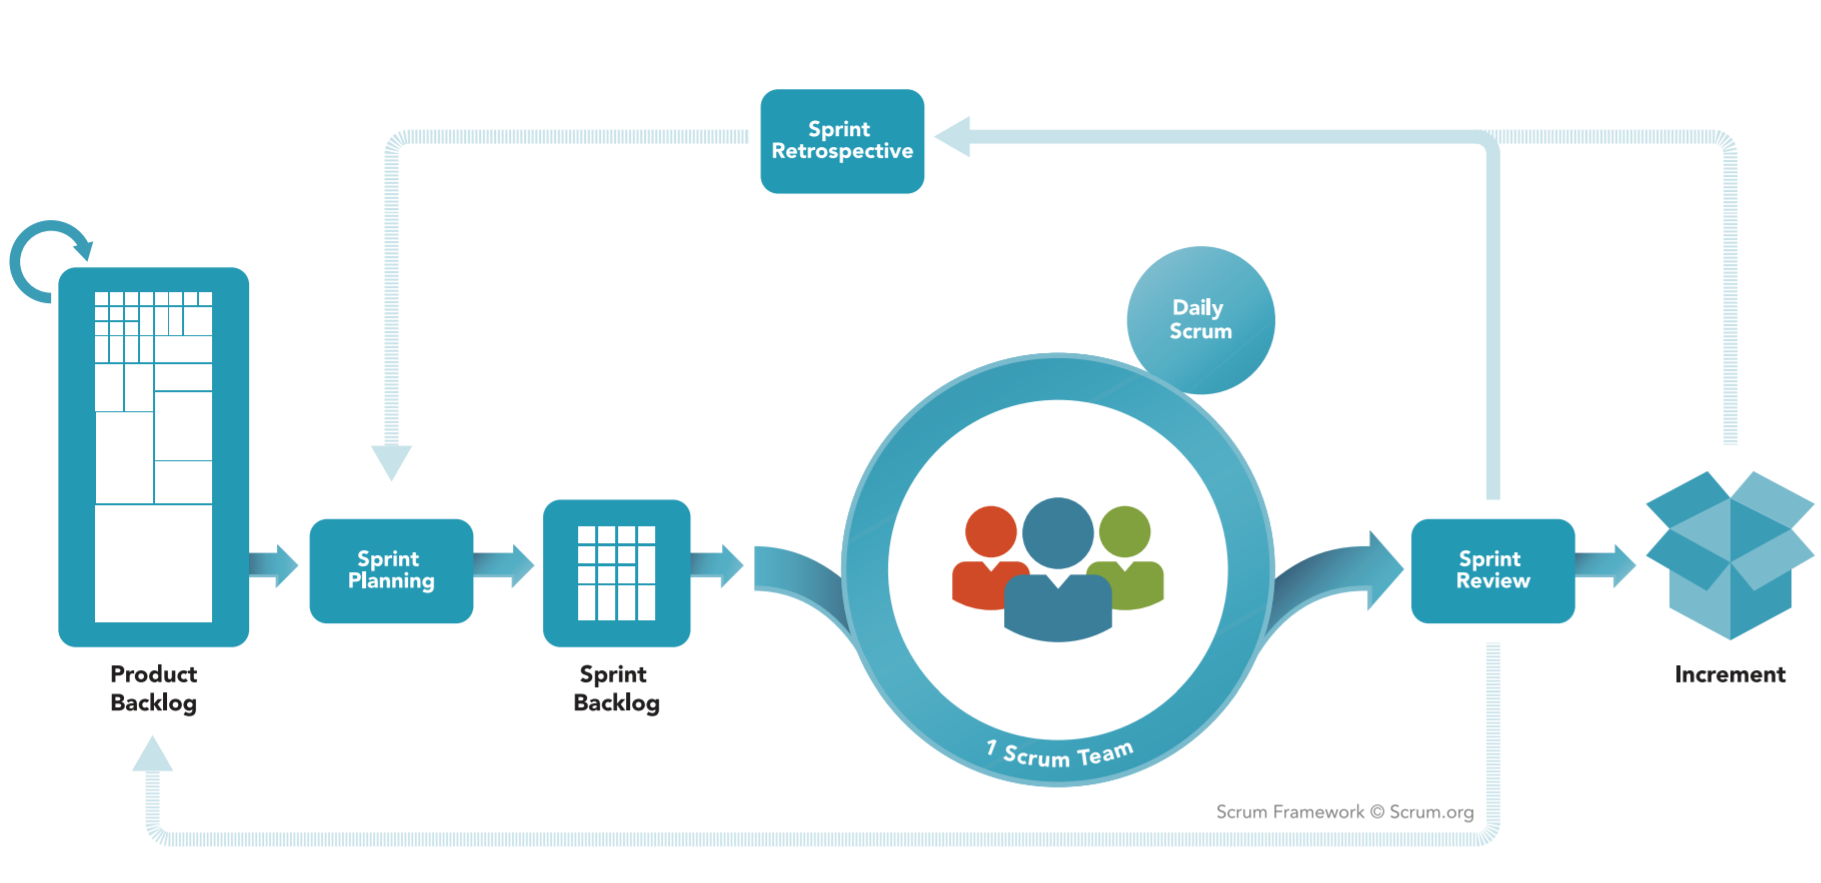
\includegraphics[width=\textwidth] {scrum.jpg}
		\caption{Metodología Scrum }
		\label{fig:scrum}
	\end{figure} 


El proceso comienza con la definición del Product Backlog, se dará pie a los futuros Sprints.
Iremos troceando Figura~\ref{fig:scrum} y comentando sus partes.
\begin{itemize}
\item \textbf{Definición del Product Backlog}\\
Es una lista con las funcionalidad de la aplicación.\\
Estas funcionalidad que se definen en el Product Owner son las historias del usuario, es decir, es lo que el usuario quiere hacer en la aplicación y por tanto en muchos casos cada historia contendrá varios casos de uso. \\
Está elaborado por el Product Owner y las funcionalidad están ordenadas de mayor a menor importancia dentro de la aplicación. La finalidad del Product Owner es plantear lo que hay que hacer.
Con las historias ordenas se indicaran los Sprints que serán necesarios pudiendo hacer  varias historias en un mismo Sprint pero nunca una historia dividida en 2 Sprints. 

 
 \begin{figure}[H]
		\centering
		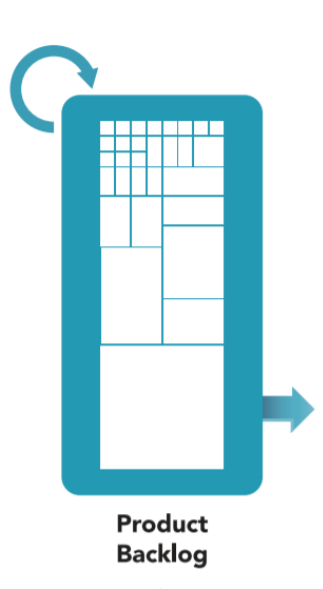
\includegraphics[width=0.2\textwidth] {product.png}
		\caption{Parte metodología Scrum, Product Backlog }\label{fig:product}
	\end{figure} 


\item \textbf{Sprint Planning Meeting}\\
 Esta reunión se hace al comienzo de cada Sprint y se define cómo se va a enfocar el proyecto que viene del Product Backlog las etapas y los plazos.
\begin{figure}[H]
		\centering
		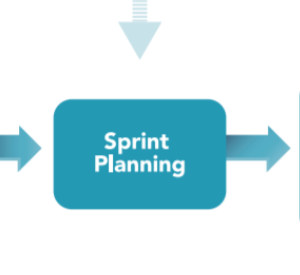
\includegraphics[width=0.3\textwidth] {planing.png}
		\caption{Parte metodología Scrum, Sprint Planning }\label{fig:planing}
	\end{figure} 

\item \textbf{Sprint Backlog}\\
Es el conjunto de historias del Product Backlog que se decidirán hacer en el Sprint, estando ordenadas de mayor a menor prioridad. Una vez hecho esto los miembros del equipo dividirán las historias en partes más pequeñas y más manejables.

\begin{figure}[H]
		\centering
		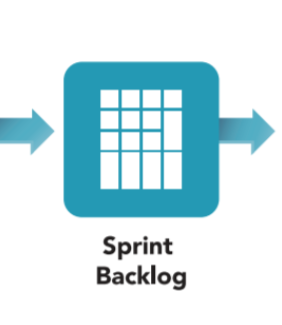
\includegraphics[width=0.3\textwidth] {sprint.png}
		\caption{Parte metodología Scrum, Sprint Backlog }\label{fig:sprint}
	\end{figure} 

 
 
\item \textbf{Daily Scrum o Stand-up Meeting}\\
Es una reunión breve que se realiza a diario mientras dura el periodo de Sprint. 
En estas reuniones si algun miembro del equipo encuentra algun problema esto se comenta y se trata de ayudarlo. Este tipo de problemas debería resolverlos el Scrum Master.

\begin{figure}[H]
		\centering
		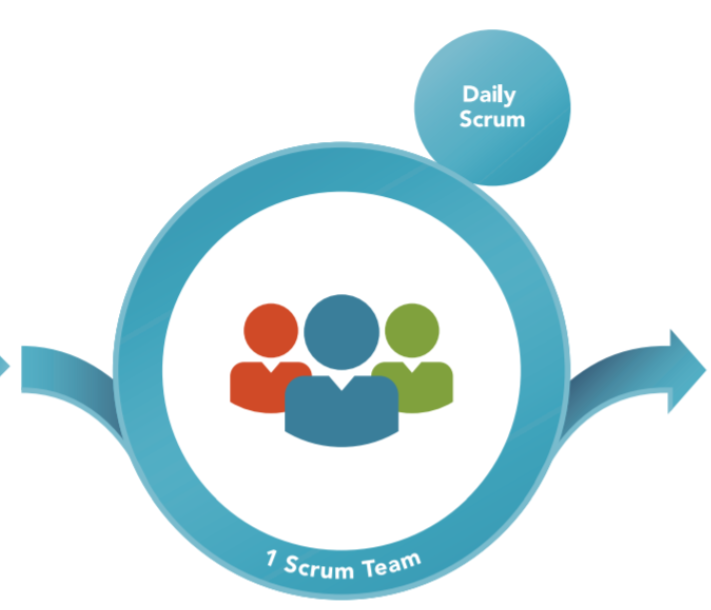
\includegraphics[width=0.3\textwidth] {daily.png}
		\caption{Parte metodología Scrum, Daily Scrum }\label{fig:daily}
	\end{figure} 

\item\textbf{ Sprint Review}\\
Esta sería la primera reunión una vez acabado el Sprint. En ella se deberían plantear las tareas acabadas y se debería ver un avance claro para ser presentado al cliente. Las tareas inacabas deberían ser devueltas al Product Backlog y si hiciera falta volver a calcular las prioridades.

 \item \textbf{Sprint Retrospective}\\
  El equipo revisa los objetivos cumplidos del Sprint terminado. Se anota lo bueno y lo malo, para no volver a repetir los errores. Esta etapa se centra en el cómo se realiza el proyecto para si hay algún error en el desarrollo poderlo resolver en el siguiente Sprint.
\end{itemize}



\section{Adaptación de este proyecto a la metodología }
 En el momento de seguir la metodología Scrum debimos realizar una serie de cambios o adaptaciones en ciertos elementos como fueron los siguientes :
\subsection{Participantes}
Los participantes fueron los siguientes:
\begin{itemize}
\item El Product Owner interpretado por los  directores.
\item El cliente tambien fue desempeñado por los directores.
\item El Scrum Master fue desempeñado por el alumno.
\item  Y el equipo solo estuvo formado por el alumno.

\end{itemize}

\subsection{Sprints}
Cada sprint siempre tuvo una duración establecida de 4 semanas y 5 horas cada día aunque la carga de trabajo variaba en algún Sprint.


\subsection{Reuniones}

En el apartado de las reuniones siempre se establecían las tareas a realizar en cada jornada de trabajo. Al finalizar cada Sprint se realizaban reuniones con los directores y se aprovechaba para la planificación de la siguiente.
